\documentclass{article}
\usepackage{pgfplots}
\pgfplotsset{compat=1.16}


\begin{document}
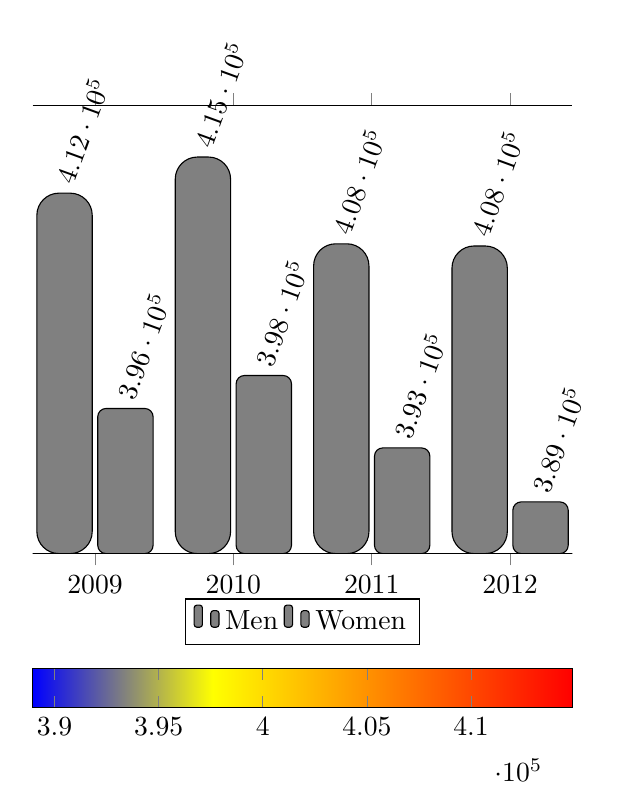
\begin{tikzpicture}
\pgfplotsset{/pgfplots/ybar legend/.style={
    /pgfplots/legend image code/.code={
        \draw [##1,/tikz/.cd,rounded corners=1pt,bar width=3pt,yshift=-0.2em,bar shift=0pt]
        plot coordinates {(0cm,0.8em) (2*\pgfplotbarwidth,0.6em)};
    },
},}         
\begin{axis}[
   hide y axis,
   colorbar horizontal,
    x tick label style={
        /pgf/number format/1000 sep=},
    ylabel=Year,
    enlargelimits=0.15,
    legend style={at={(0.5,-0.1)}, anchor=north,legend columns=-1},
    ybar,bar width=2em,
    ybar legend,
    nodes near coords=\pgfmathprintnumber{\pgfplotspointmeta},
    every node near coord/.append style={
    anchor=mid west,
    rotate=70}
]
\addplot[rounded corners=8pt,fill=gray] 
    coordinates {(2012,408184) (2011,408348)
        (2010,414870) (2009,412156)};
\addplot[rounded corners=3pt,fill=gray]  
    coordinates {(2012,388950) (2011,393007) 
        (2010,398449) (2009,395972)};
\legend{Men,Women}
\end{axis}
\end{tikzpicture}
\end{document}